% This is based on the LLNCS.DEM the demonstration file of
% the LaTeX macro package from Springer-Verlag


\documentclass{llncs}

\usepackage{graphicx}

\usepackage{hyperref}
\usepackage{placeins}

\usepackage{listings}
\usepackage{color}

% \graphicspath{ {images/} }
\pagestyle{plain}


\definecolor{dkgreen}{rgb}{0,0.6,0}
\definecolor{gray}{rgb}{0.5,0.5,0.5}
\definecolor{mauve}{rgb}{0.58,0,0.82}

\lstset{frame=tb,
  language=Java,
  aboveskip=3mm,
  belowskip=3mm,
  showstringspaces=false,
  columns=flexible,
  basicstyle={\small\ttfamily},
  numbers=none,
  numberstyle=\tiny\color{gray},
  keywordstyle=\color{blue},
  commentstyle=\color{dkgreen},
  stringstyle=\color{mauve},
  breaklines=true,
  breakatwhitespace=true,
  tabsize=3
}


\begin{document}

\title{GridAdmin}
%
\titlerunning{GridAdmin}  % abbreviated title (for running head)
%                                     also used for the TOC unless
%                                     \toctitle is used
% \inst{1}
\author{Dan Alexandru}
%
\authorrunning{Dan Alexandru} % abbreviated author list (for running head)
%
%%%% list of authors for the TOC (use if author list has to be modified)
\tocauthor{Dan Alexandru}
%
\institute{Faculty of Computer Science, Iasi, Romania\\
\email{dan.alexandru@info.uaic.ro},\\ web home page:
\texttt{https://github.com/xR86/rc-project}
}

\maketitle              % typeset the title of the contribution
%


%
\begin{abstract}
GridAdmin offers a solution for orchestration of VMs - both on managed servers and cloud servers (like AWS), with a client-server architecture, the server acting as a command and control server, and the client offering a web interface.\dots
\keywords{networking, Linux, C, Python, AWS}
\end{abstract}
%

\section{Introduction}
%
GridAdmin offers a solution for network administration by sending commands through a Python GUI to a C intermediary server that passes along data to the Python server, that uses ssh to pass the commands to the slave machines (or respective API available for cloud platforms).
\\\\
Targeted functionality similar to Python's Fabric (\url{http://www.fabfile.org/}).

%
\section{Technologies used}
%

\subsection{Server-side}

The project uses C for the concurrent TCP server. Use of libssh (\url{https://www.libssh.org/}) can be employed on the server (master), along with openssh-server on the slave, but since libssh is unstable/not functional with certain OS/openssh versions, it will require the use of the Paramiko ssh library.\\
If needed, the C server could be extended with python modules.

\subsection{Client-side}

The project uses Python and PyQt4, the interface being modeled with web technologies such as HTML, CSS, Javascript, Angular.js. This will grant easier interface creation, and a more rich interface, (example of frameworks doing this: Apache Cordova - \url{https://cordova.apache.org/} / Ionic, Electron). One example of web app that runs on desktop is Slack (\url{https://slack.com/downloads/windows}).

\begin{figure}[!h]
	\label{fig:example}
	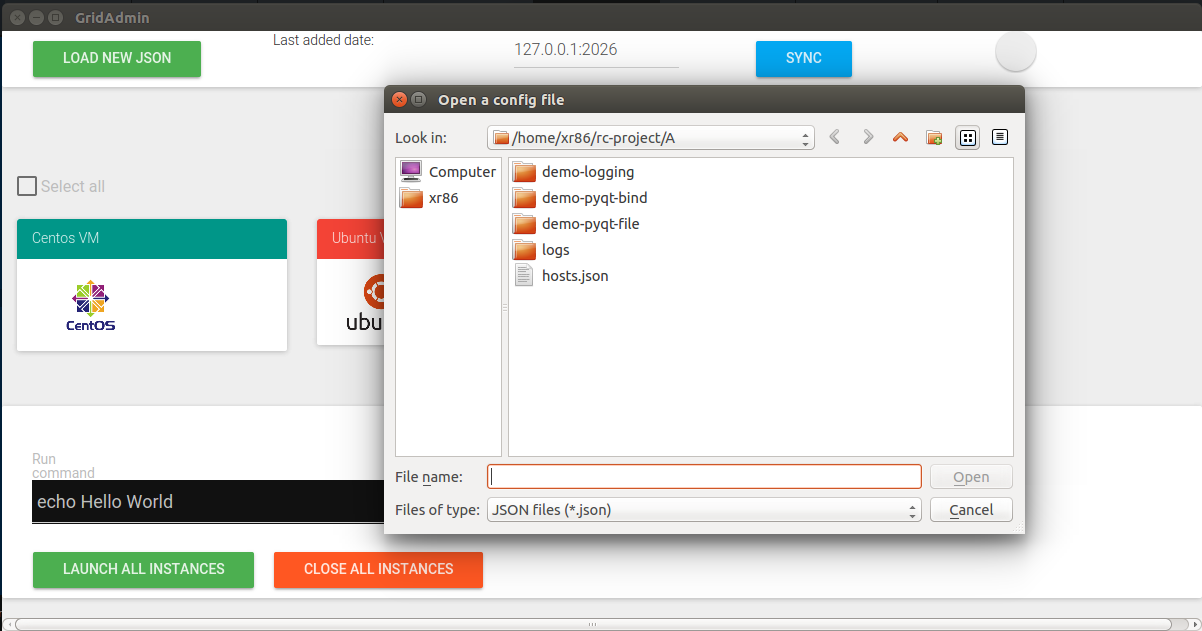
\includegraphics[scale=0.35]{client-interm.png}
	\centering
	\caption{Client demo}
\end{figure}

\FloatBarrier
%
\section{Application Architecture}
%
The application makes use of the client-server model for interfacing and master-slave model for control.

\subsection{Client-server model}
In this project, the \textbf{client} is the Python GUI that can be remote or on the same machine as the server. The client connects to the C \textbf{server} to run bulk commands (to multiple machines) or to run one or more commands on one machine.\\
The server will ssh to various machines, execute commands from client and return the output to the client.

\subsection{Master-slave model}
In this project, the \textbf{master-slave model} acknowledges that there is a server that has ssh access to various machines (public-key authentication and/or password authentication), and can run almost anything on them (if root mode allowed in \textbf{sshd\_config}).

\subsection{Application layer diagram}


\begin{figure}[!ht]
\includegraphics[scale=0.45]{new_ideal_app_layer.png}
\centering
\caption{Redesigned Application Layer architecture - The client exchanges data with the server, that is C and Python separately (C data proxy and Python Paramiko server)}, the server then connects either to various machines (with openssh pre-installed) or to a AWS EC2 instance (through the API).
\end{figure}


\begin{figure}[!ht]
\includegraphics[scale=0.45]{new_automata.png}
\centering
\caption{Automata for GridAdmin.}
\end{figure}

\FloatBarrier
%
\section{Implementation details}
%

\subsection{Application flow}

\iffalse %start comment

The application flow is:
\begin{itemize}
  \item user deploys various instances/servers
  \item user saves a config file and deploys the master server. The config file will contain \textbf{IP:user:password/pubkeyName}, and may contain the following machine types:
  \begin{itemize}
  	\item containers (eg: Docker)
    \item VMs - ssh to host, then use VBoxManage to port forward (and/or use bridged mode) and make a mapping (and use the API) between forwarded ports and desired VMs (eg: \textbf{VBoxManage modifyvm rc-box1 --natpf1 "ssh,tcp,,3022,,22"} - for VM called "rc-box1", forward guest port 22 to host port 3022 ) - automated through Vagrant
    \item servers
    \item EC2 instances (or equivalent)
  \end{itemize}
  \item user then opens the GUI client, and checks initially the status of all the machines in the config file
  \item master server runs: \textbf{ssh-copy-id \textless remoteuser\textgreater@\textless remotehostIP \textgreater} (meaning, it exchanges keys with the remote slaves, so it could establish the ssh connection later)
  \item master server checks the status of the machines
  \item after this, you could send various commands within the interface to selected machines, and have the differentiated output and logs sent back to you
\end{itemize}

\fi %end comment

\subsection{Relevant code}

\iffalse %start comment

Some of the relevant code snippets for this project will be explained here.\\

The work will be split in 3 parts
\begin{itemize}
	\item client
    \item server and configs (e.g.: \textbf{sshd\_config} file)
    \item automatization (Vagrant, APIs, supporting different archetypes of machines)
\end{itemize}

\begin{figure}
\begin{lstlisting}[language=Ruby]
# establishing VM variables
api_version = '2'
provider    = 'virtualbox'
box         = 'ubuntu/trusty64'
hostname    = 'rc-box'
ip          = '192.168.50.13'
ram         = '2048'

# configuring Vagrant deployment
Vagrant.configure(api_version) do |config|
  	# configure variable
  	config.vm.define "rc" do |rc|
	end

	# creating new VM with specified parameters
	config.vm.box = box
	config.vm.host_name = hostname
	config.vm.network :private_network, ip: ip
end
\end{lstlisting}
	\centering
	\caption{Vagrantfile snippet - automating VM deployment}
\end{figure}

\begin{figure}
\begin{lstlisting}[language=C]
int main() {

    ssh_session session; // creates a new session (connection)
    ssh_channel channel; // creates a new channel (data)
    int rc, port = 22; //status flag and port variable
    char buffer[1024]; //buffer for ssh responses
    unsigned int nbytes; //

    printf("Session...\n");
    session = ssh_new();
    if (session == NULL) exit(-1);

    ssh_options_set(session, SSH_OPTIONS_HOST, "localhost"); //localhost //192.168.100.2
    ssh_options_set(session, SSH_OPTIONS_PORT, &port);
    ssh_options_set(session, SSH_OPTIONS_USER, "xR86"); //xR86 //labsi

    printf("Connecting...\n");
    rc = ssh_connect(session);
    if (rc != SSH_OK) error(session);

    printf("Password Autentication...\n");
    //rc = ssh_userauth_password(session, "NULL", "password"); // second is username, third is password
    rc = ssh_userauth_publickey_auto(session, "xR86", NULL); //automatically looks in .ssh/ keys
    if (rc != SSH_AUTH_SUCCESS) error(session); // if auth fails, the program stops here

    printf("Channel...\n");
    channel = ssh_channel_new(session); //connection established
    if (channel == NULL) exit(-1);

    printf("Opening...\n");
    rc = ssh_channel_open_session(channel);
    if (rc != SSH_OK) error(session);

    printf("Executing remote command...\n");
    rc = ssh_channel_request_exec(channel, "ls -l"); //system call in remote machine
    if (rc != SSH_OK) error(session); //cmd failed

    printf("Received:\n");
    nbytes = ssh_channel_read(channel, buffer, sizeof(buffer), 0);
    while (nbytes > 0) {
        fwrite(buffer, 1, nbytes, stdout);
        nbytes = ssh_channel_read(channel, buffer, sizeof(buffer), 0);
    }

    free_channel(channel); //EOF, close and deallocate
    free_session(session); //disconnect and deallocate memory

    return 0;
}
\end{lstlisting}
	\centering
	\caption{C libssh snippet}
\end{figure}


\FloatBarrier

\fi %end comment

%
\section{Conclusions}
%

The solution could be extended to be: 

\begin{itemize}
  \item \textbf{cloud provider agnostic} (especially IaaS), offering support for Google Cloud Platform and/or Microsoft Azure)
  \item duplicating the \textbf{server and hosting it in different geographical locations} and infrastructure backbones - for availability / legal reasons
  \item offering \textbf{specific commands in the interface} such as on-the-fly snapshots, backup rotation of logs (backup rotation scheme), bulk close/sleep/open, grouping after type (VM/instance/etc)
\end{itemize}

.
%
\\
\\
\\
Solution will be made available at the following address:
 \begin{center}\url{https://github.com/xR86/rc-project}\end{center}

\end{document}
